
The same figures have been generated for a 25-antenna array where the spacings were still equal but the grid of antennas is made from equilateral triangles. This reduces the spacing between the rows but also enlargens the array towards the left and right. This ``squishing'' effect can also be seen in the radiation patterns. The geometry can be seen in figure \ref{fig:equilat-geometry}.\\

The same principle regarding the spacing, grating lobes and beamwidth as in the square array case applies. However, the grating lobes along the $u$-direction are farther away and so appear at a greater angle.

\begin{figure}[h]
    \centering
    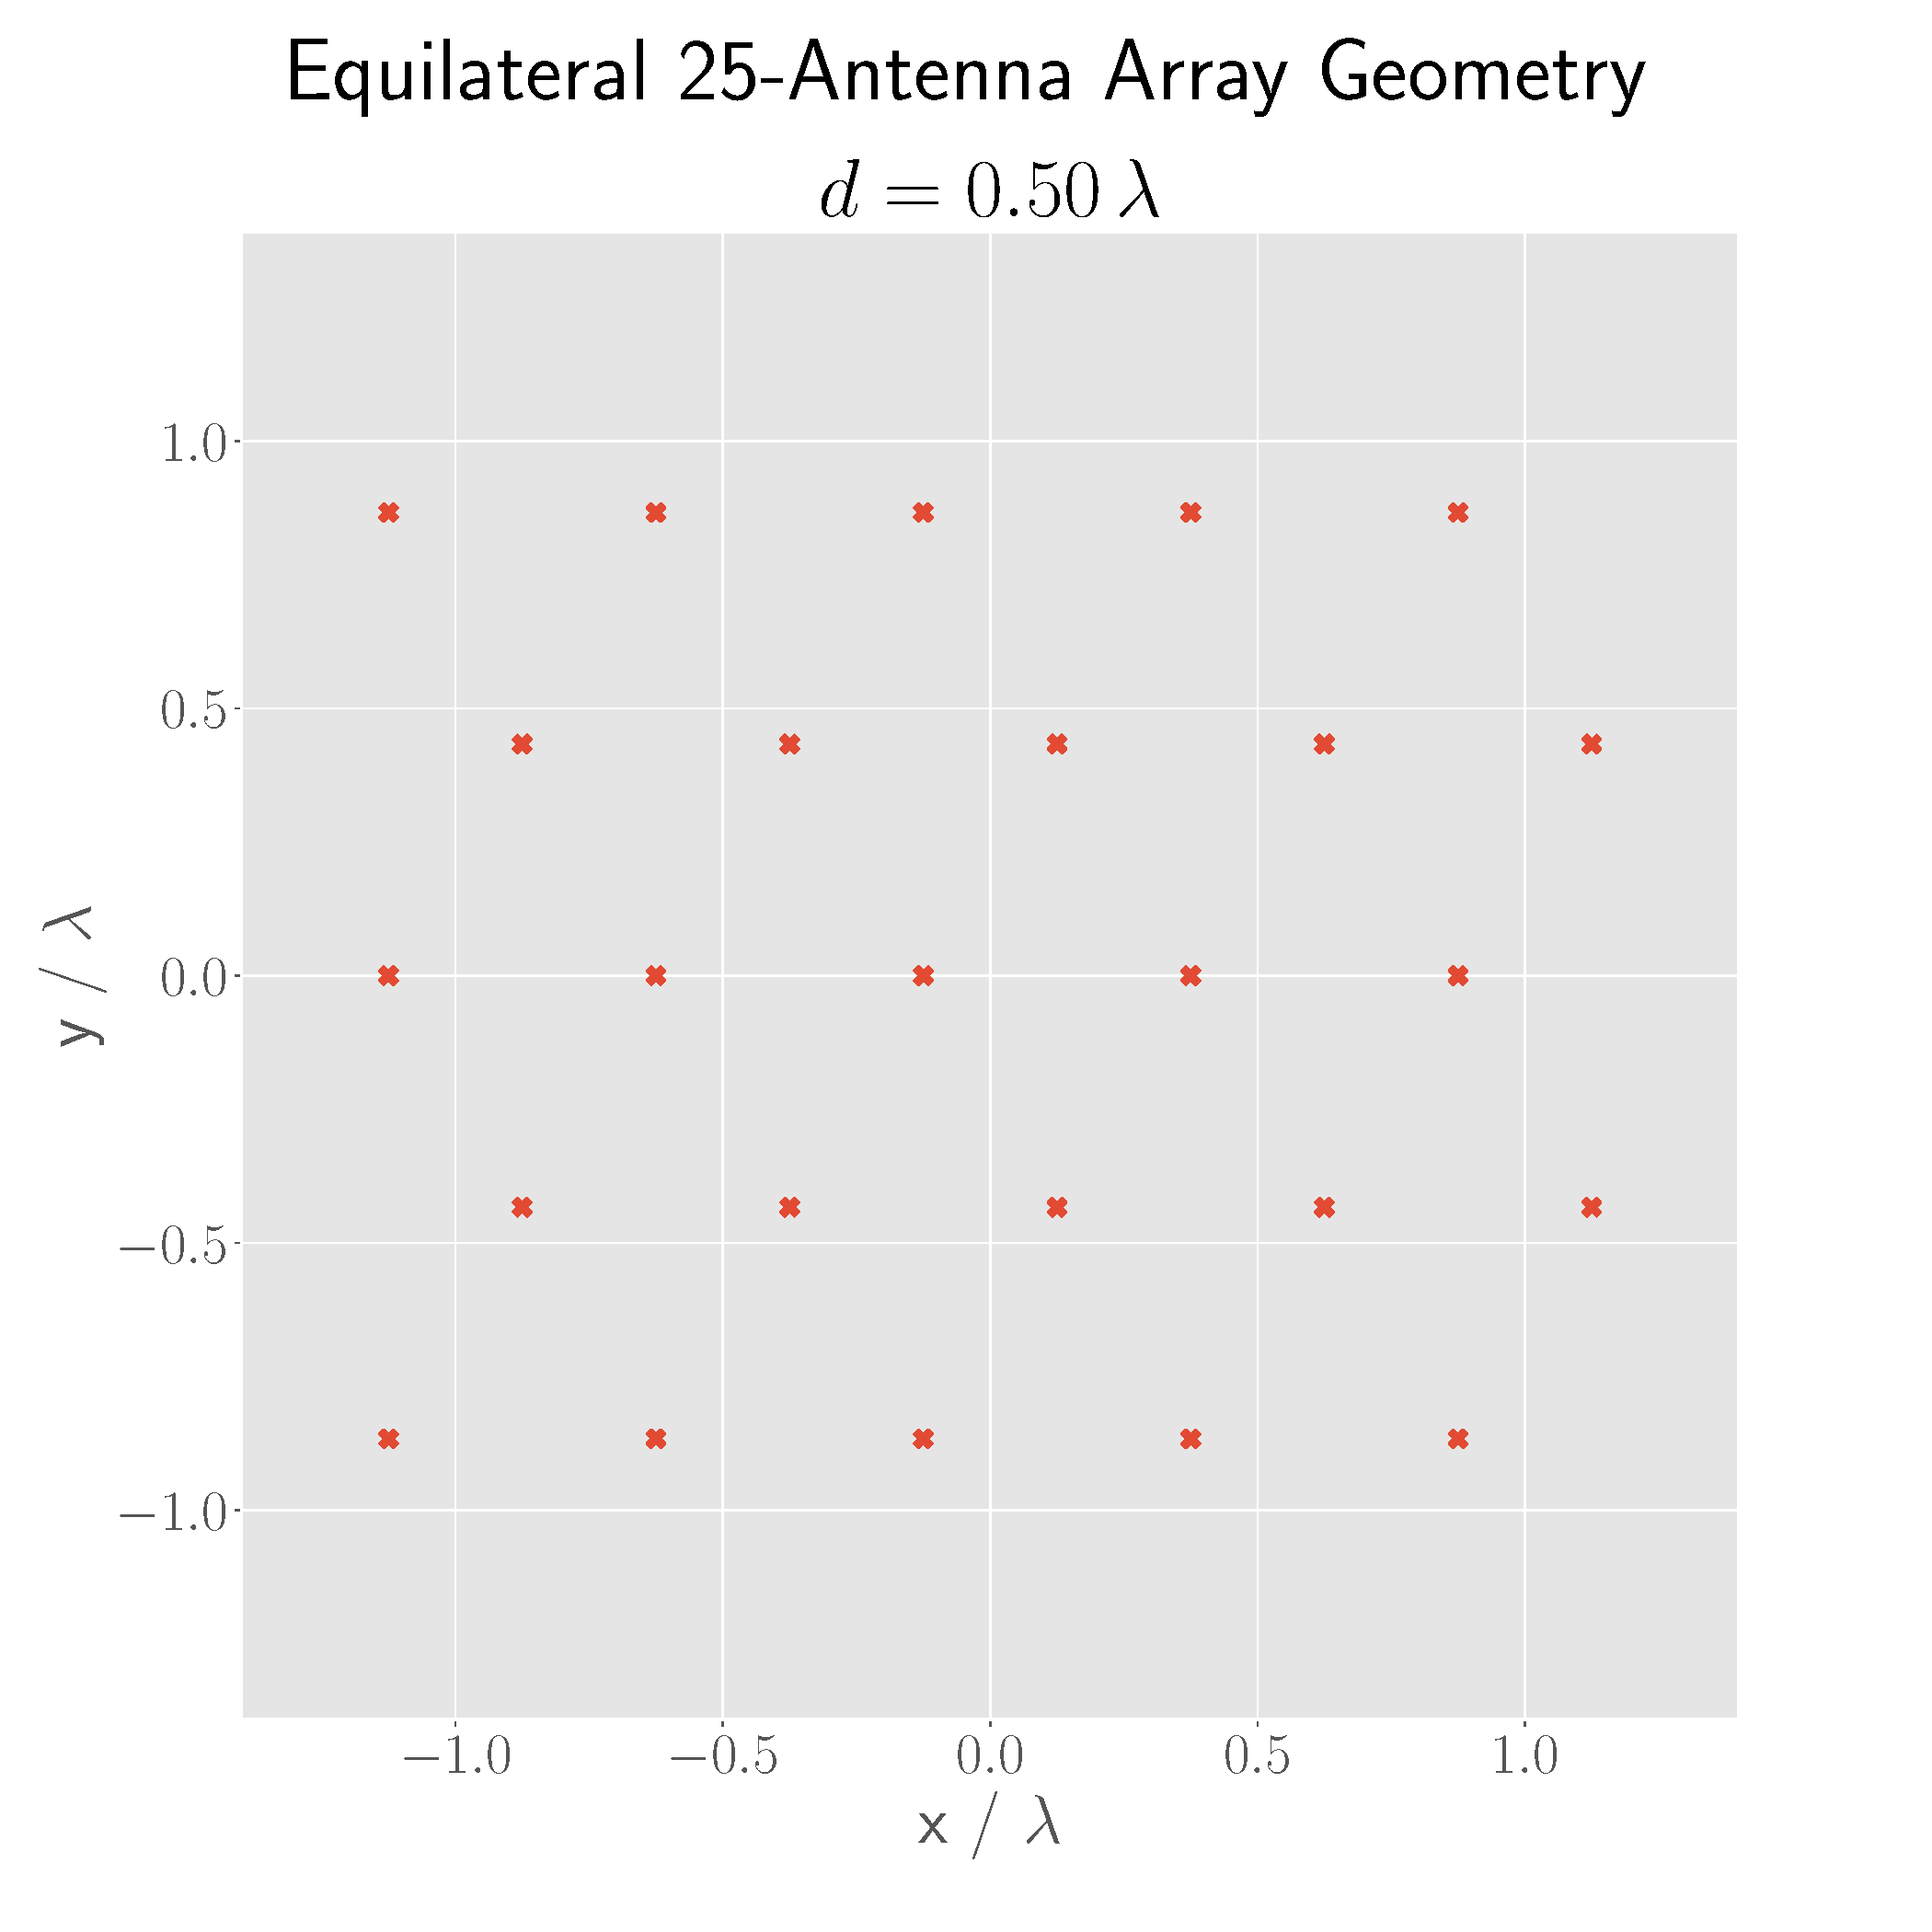
\includegraphics[width=0.4\textwidth]{graphics/task_3/equilat-0.50-lambda-0.00-theta-0.00-phi-geometry.pdf}
    \caption{Equilateral grid array structure for $d=0.5\,\lambda$}\label{fig:equilat-geometry}
\end{figure}

\begin{figure}[H]
  \begin{minipage}[t]{0.45\textwidth}
    \centering
    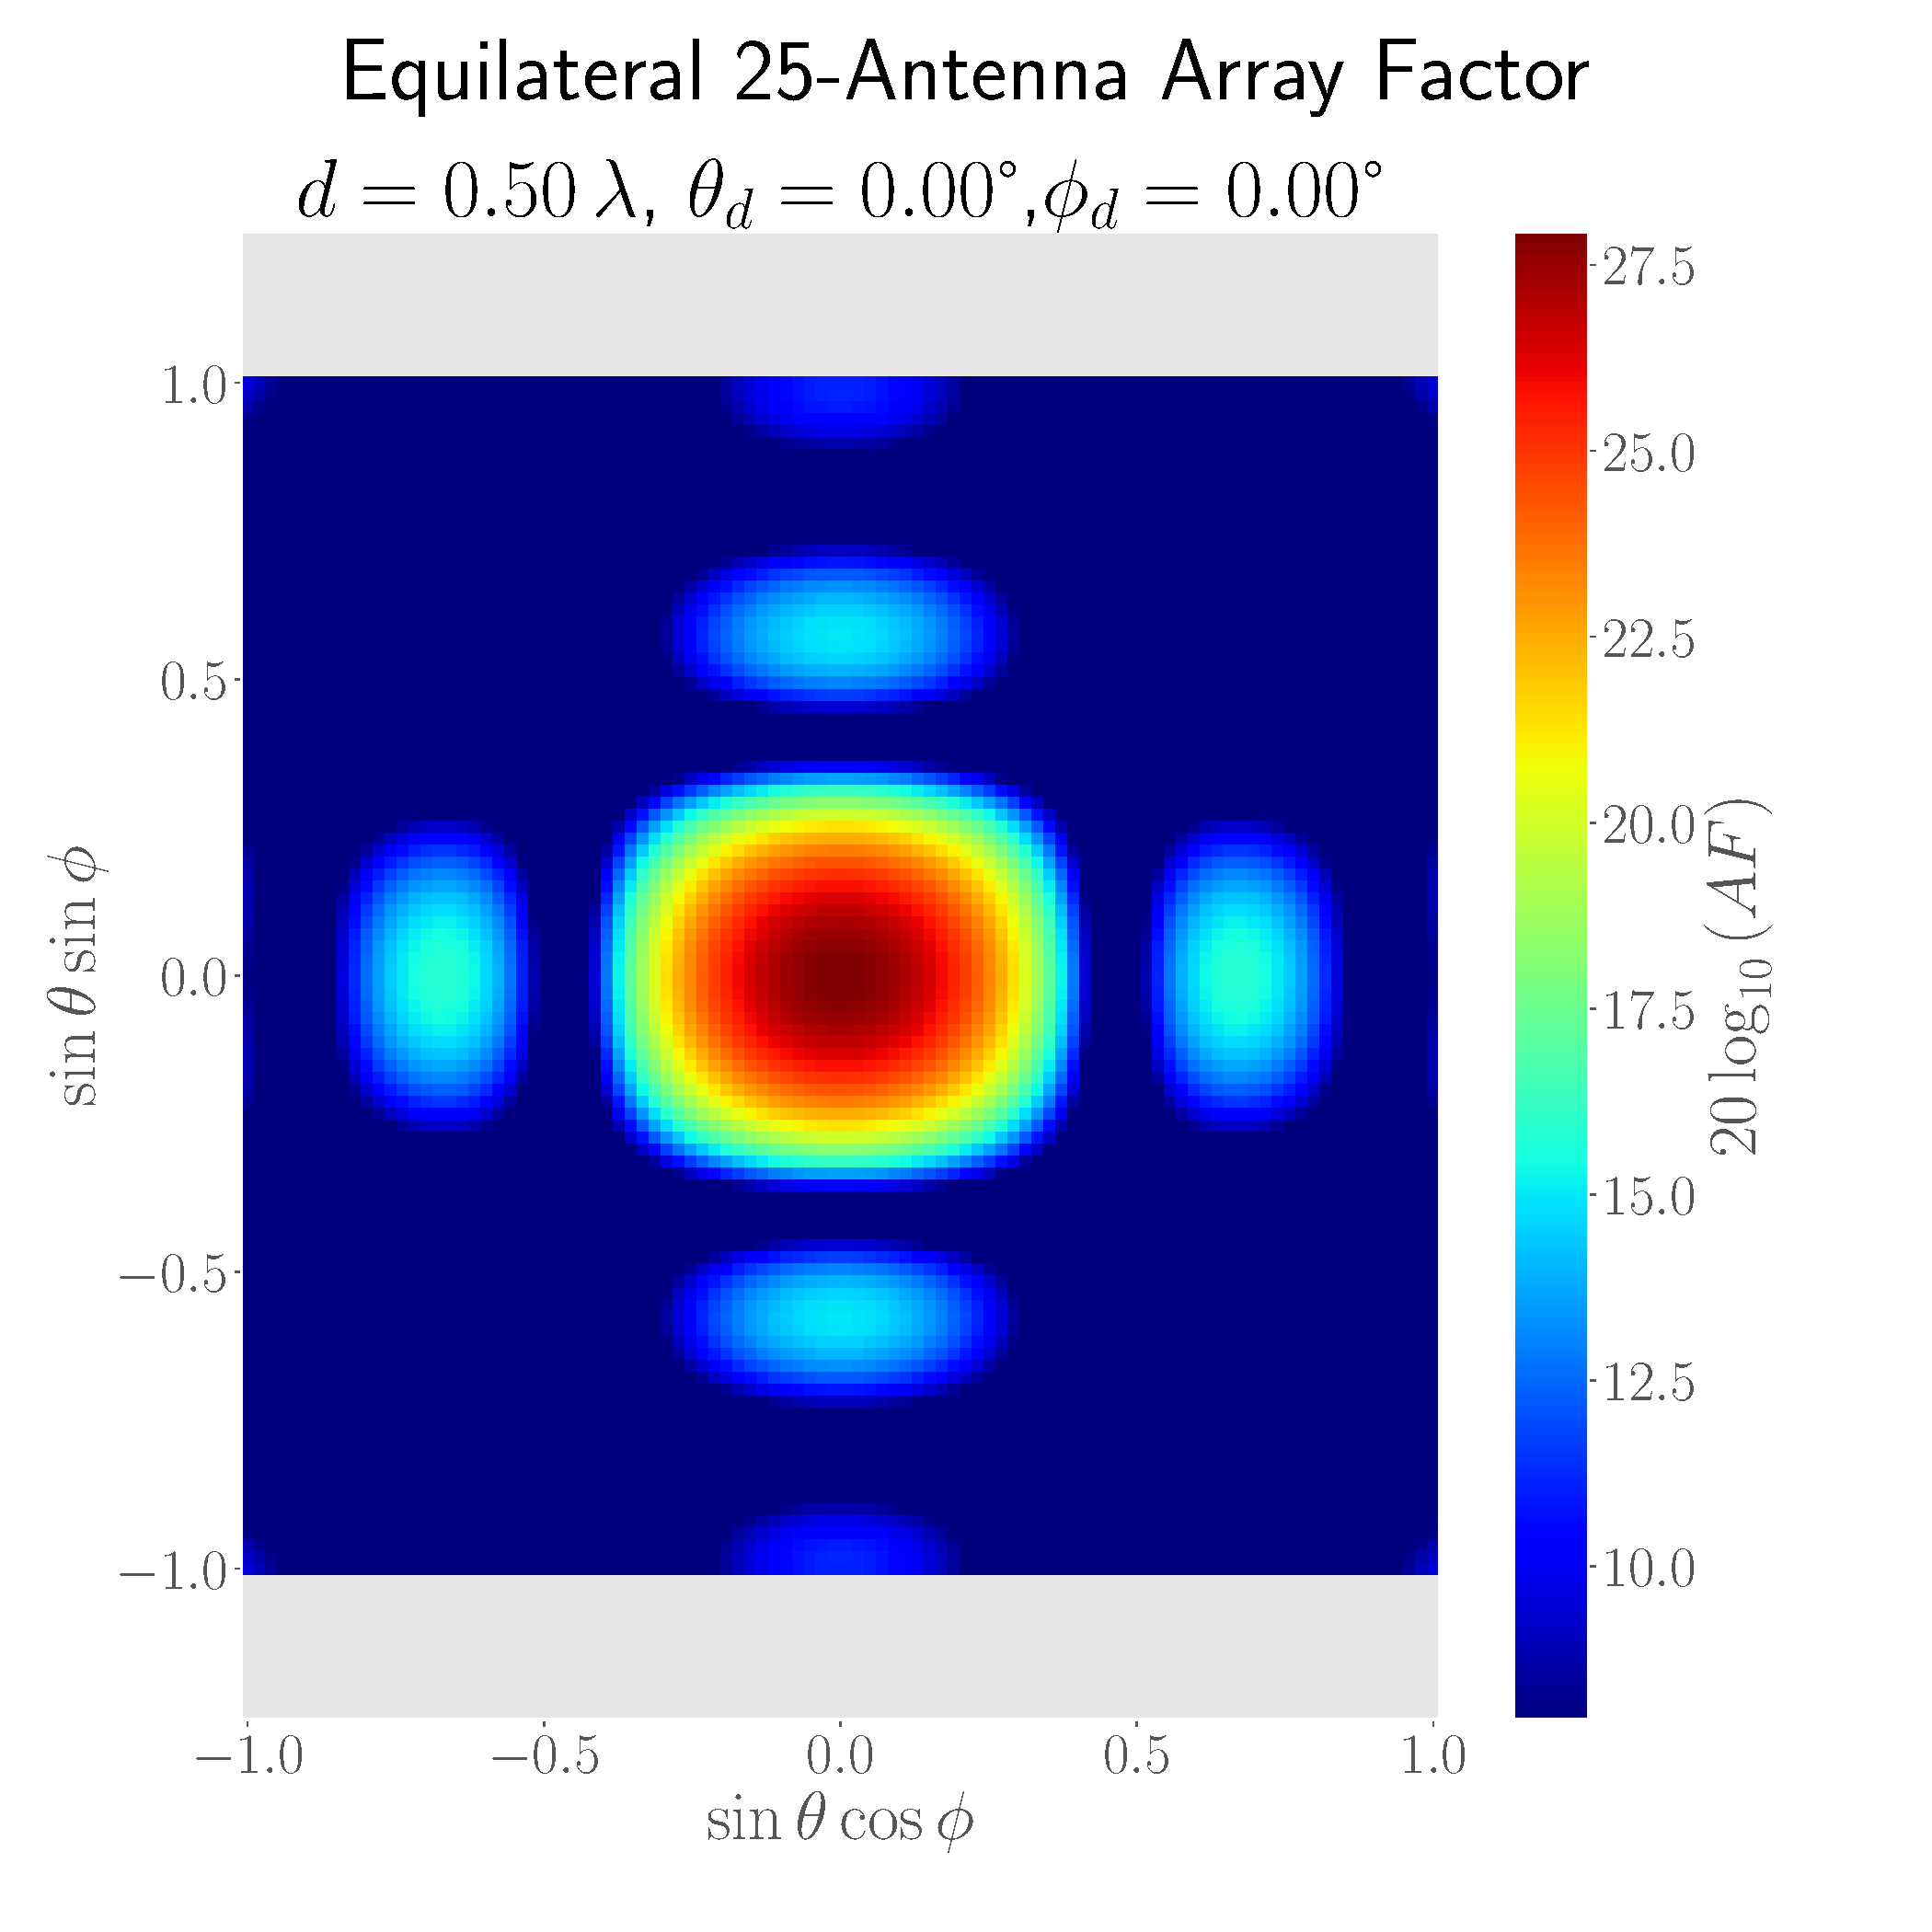
\includegraphics[width=\textwidth]{graphics/task_3/equilat-0.50-lambda-0.00-theta-0.00-phi-radpat.pdf}
    \caption{Equilateral vertically steered radiation pattern for $0.5\lambda$ spacing.}\label{fig:rad-equilat-0.5-0}
  \end{minipage}\hfill
  \begin{minipage}[t]{0.45\textwidth}
    \centering
    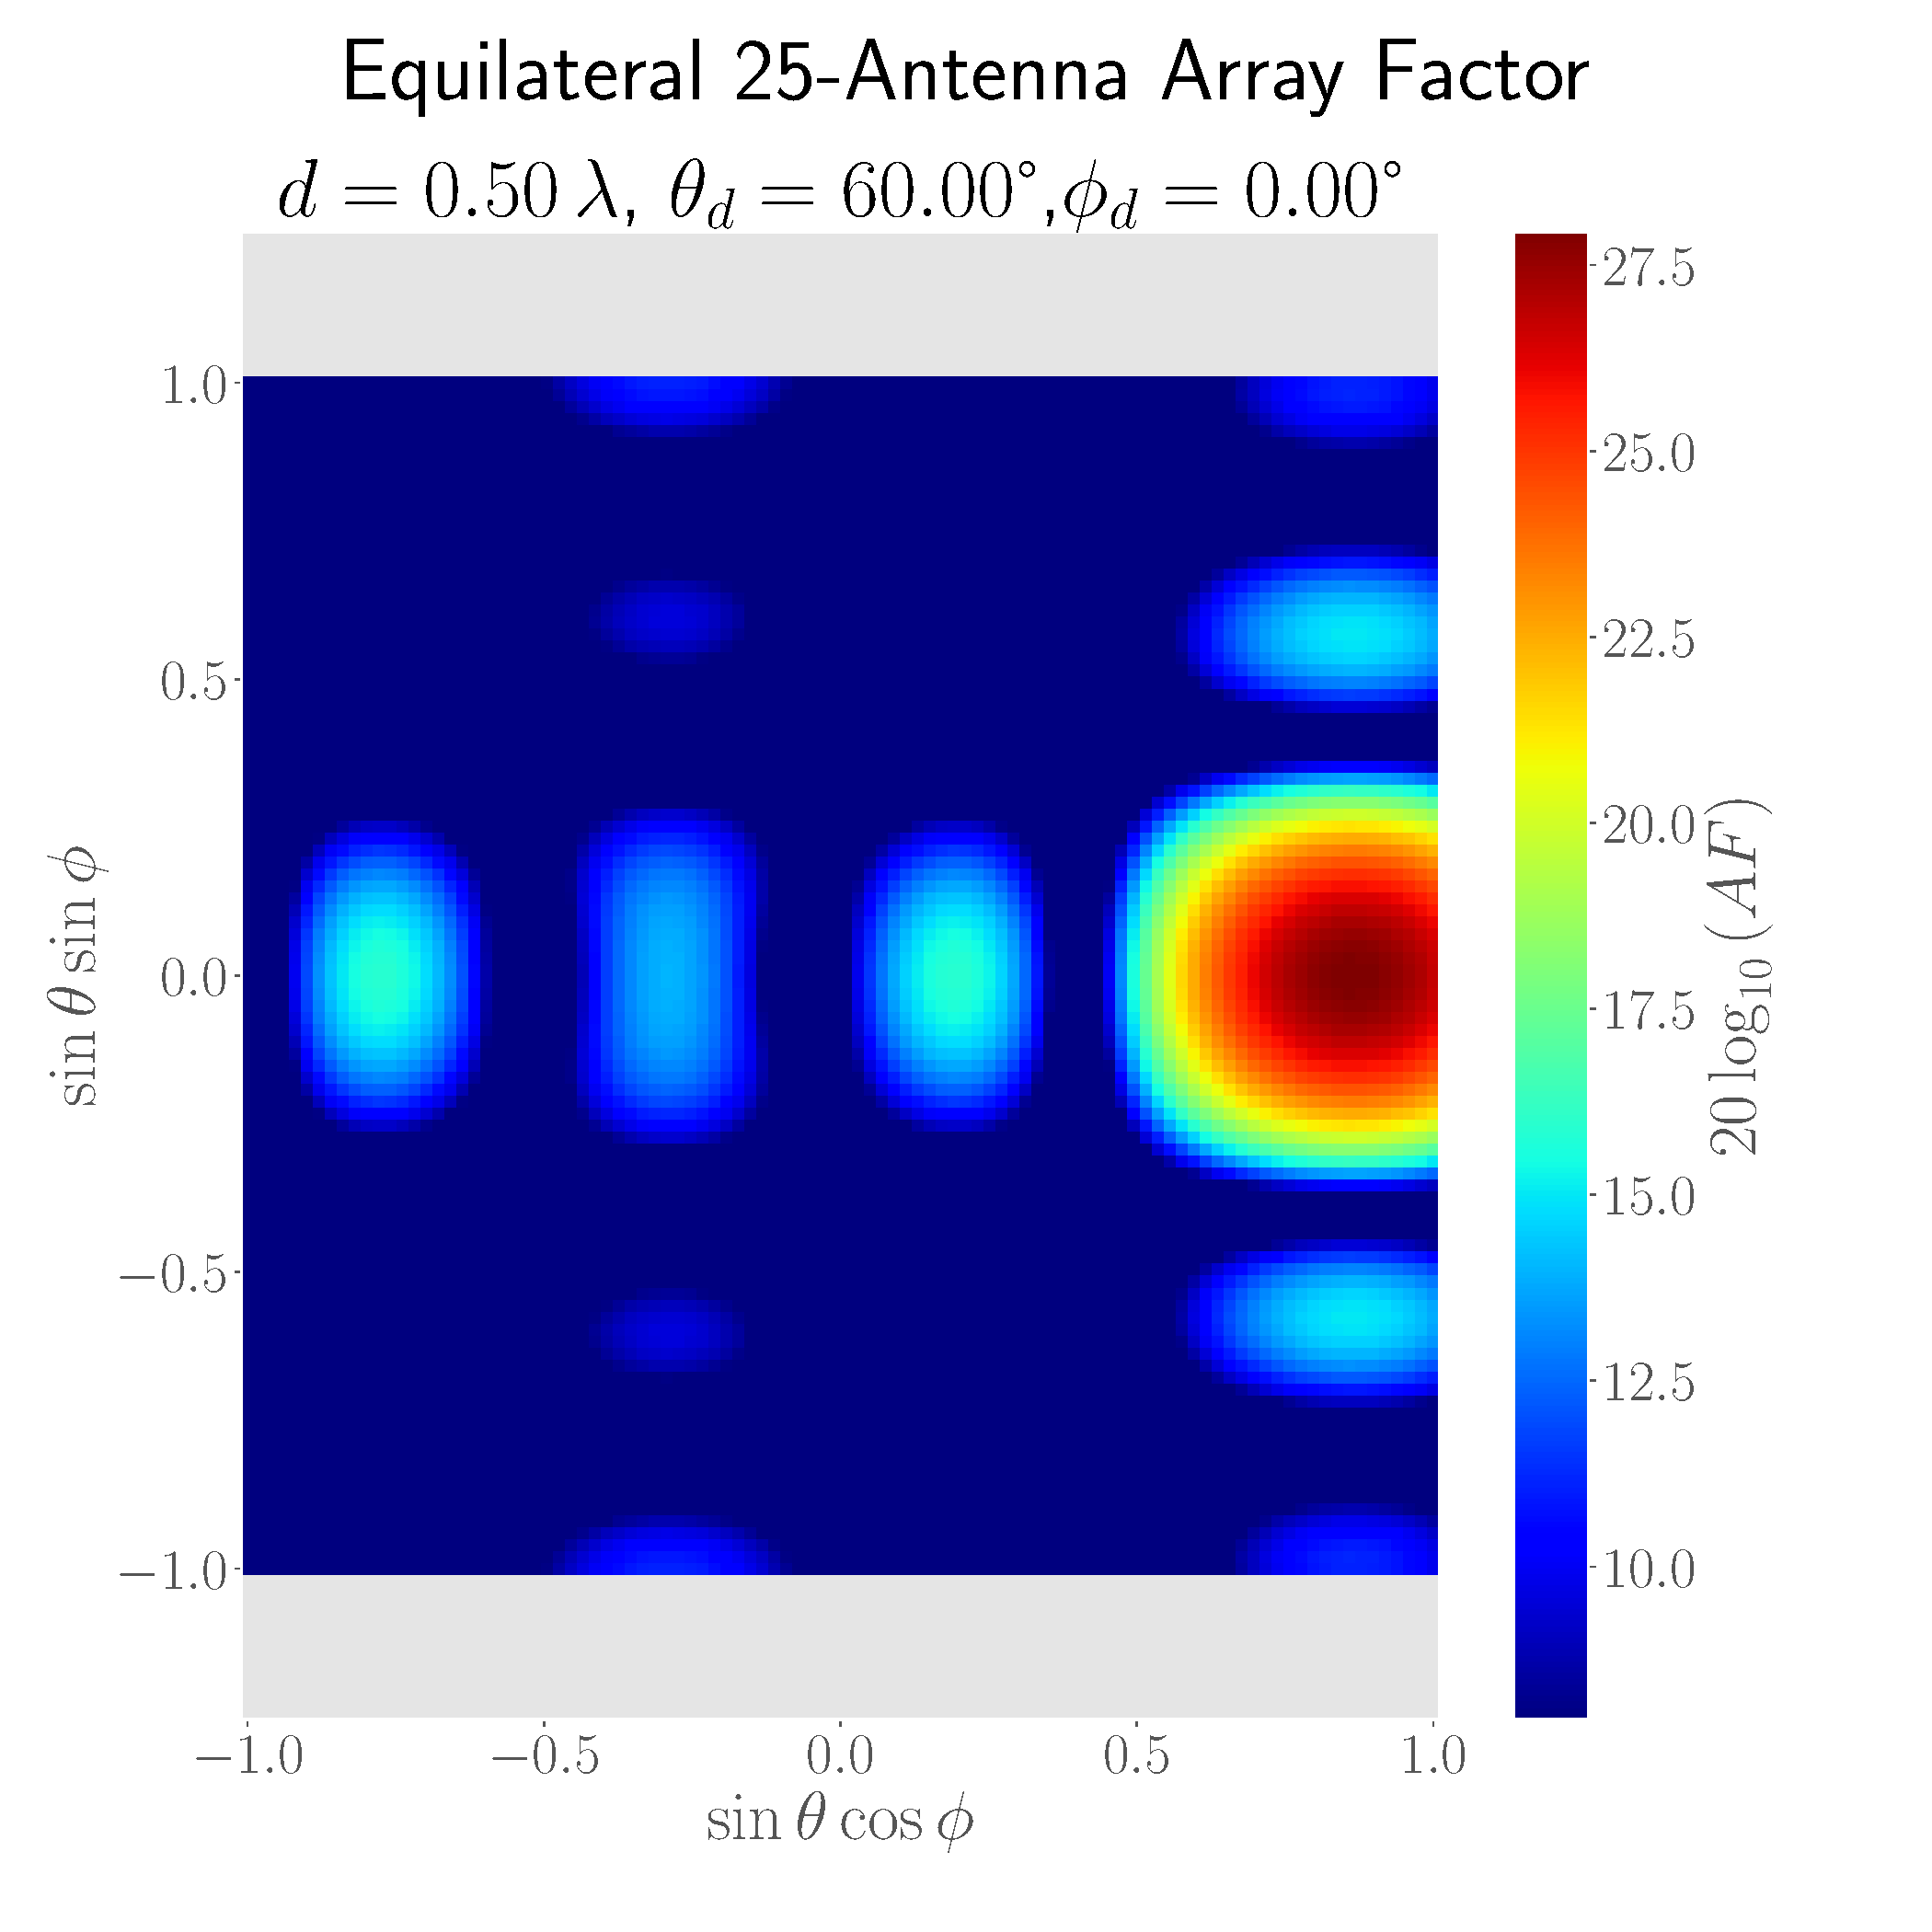
\includegraphics[width=\textwidth]{graphics/task_3/equilat-0.50-lambda-60.00-theta-0.00-phi-radpat.pdf}
    \caption{Equilateral off-vertically steered radiation pattern for $0.5\lambda$ spacing.}\label{fig:rad-equilat-0.5-60}
   \end{minipage}
\end{figure}

\begin{figure}[H]
  \begin{minipage}[t]{0.45\textwidth}
    \centering
    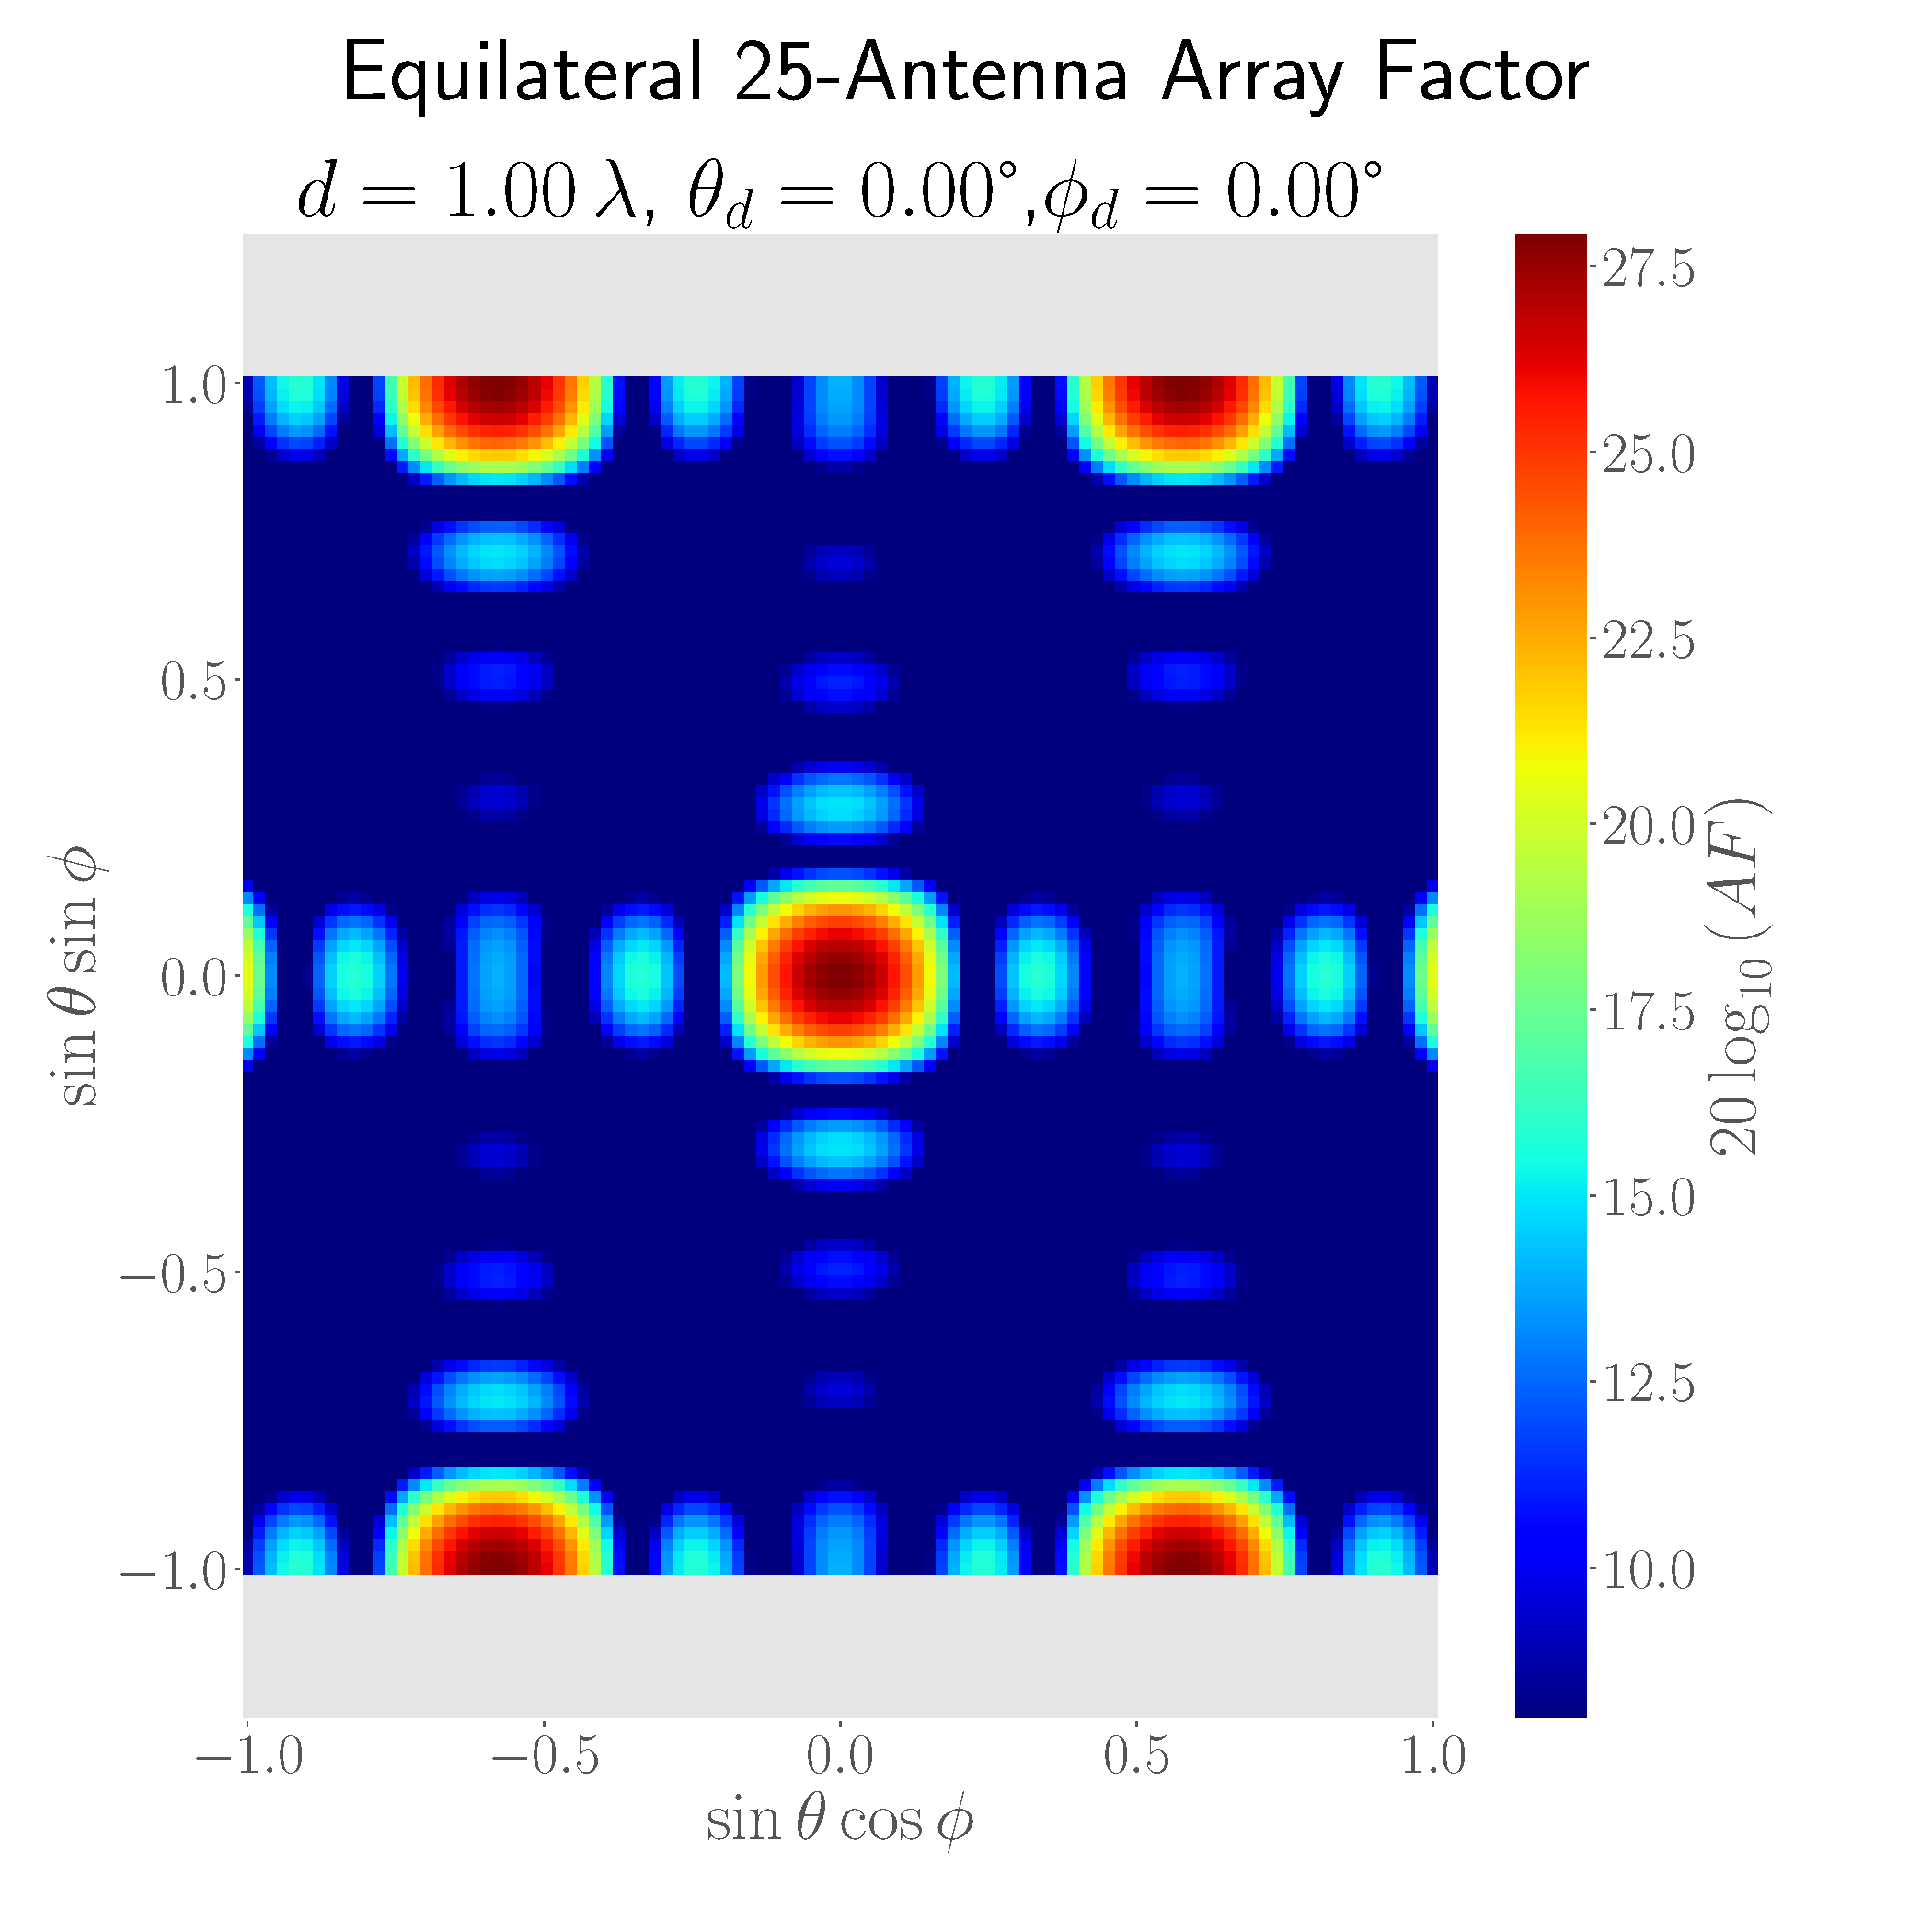
\includegraphics[width=\textwidth]{graphics/task_3/equilat-1.00-lambda-0.00-theta-0.00-phi-radpat.pdf}
    \caption{Equilateral vertically steered radiation pattern for $1.0\lambda$ spacing.}\label{fig:rad-equilat-1.0-0}
  \end{minipage}\hfill
  \begin{minipage}[t]{0.45\textwidth}
    \centering
    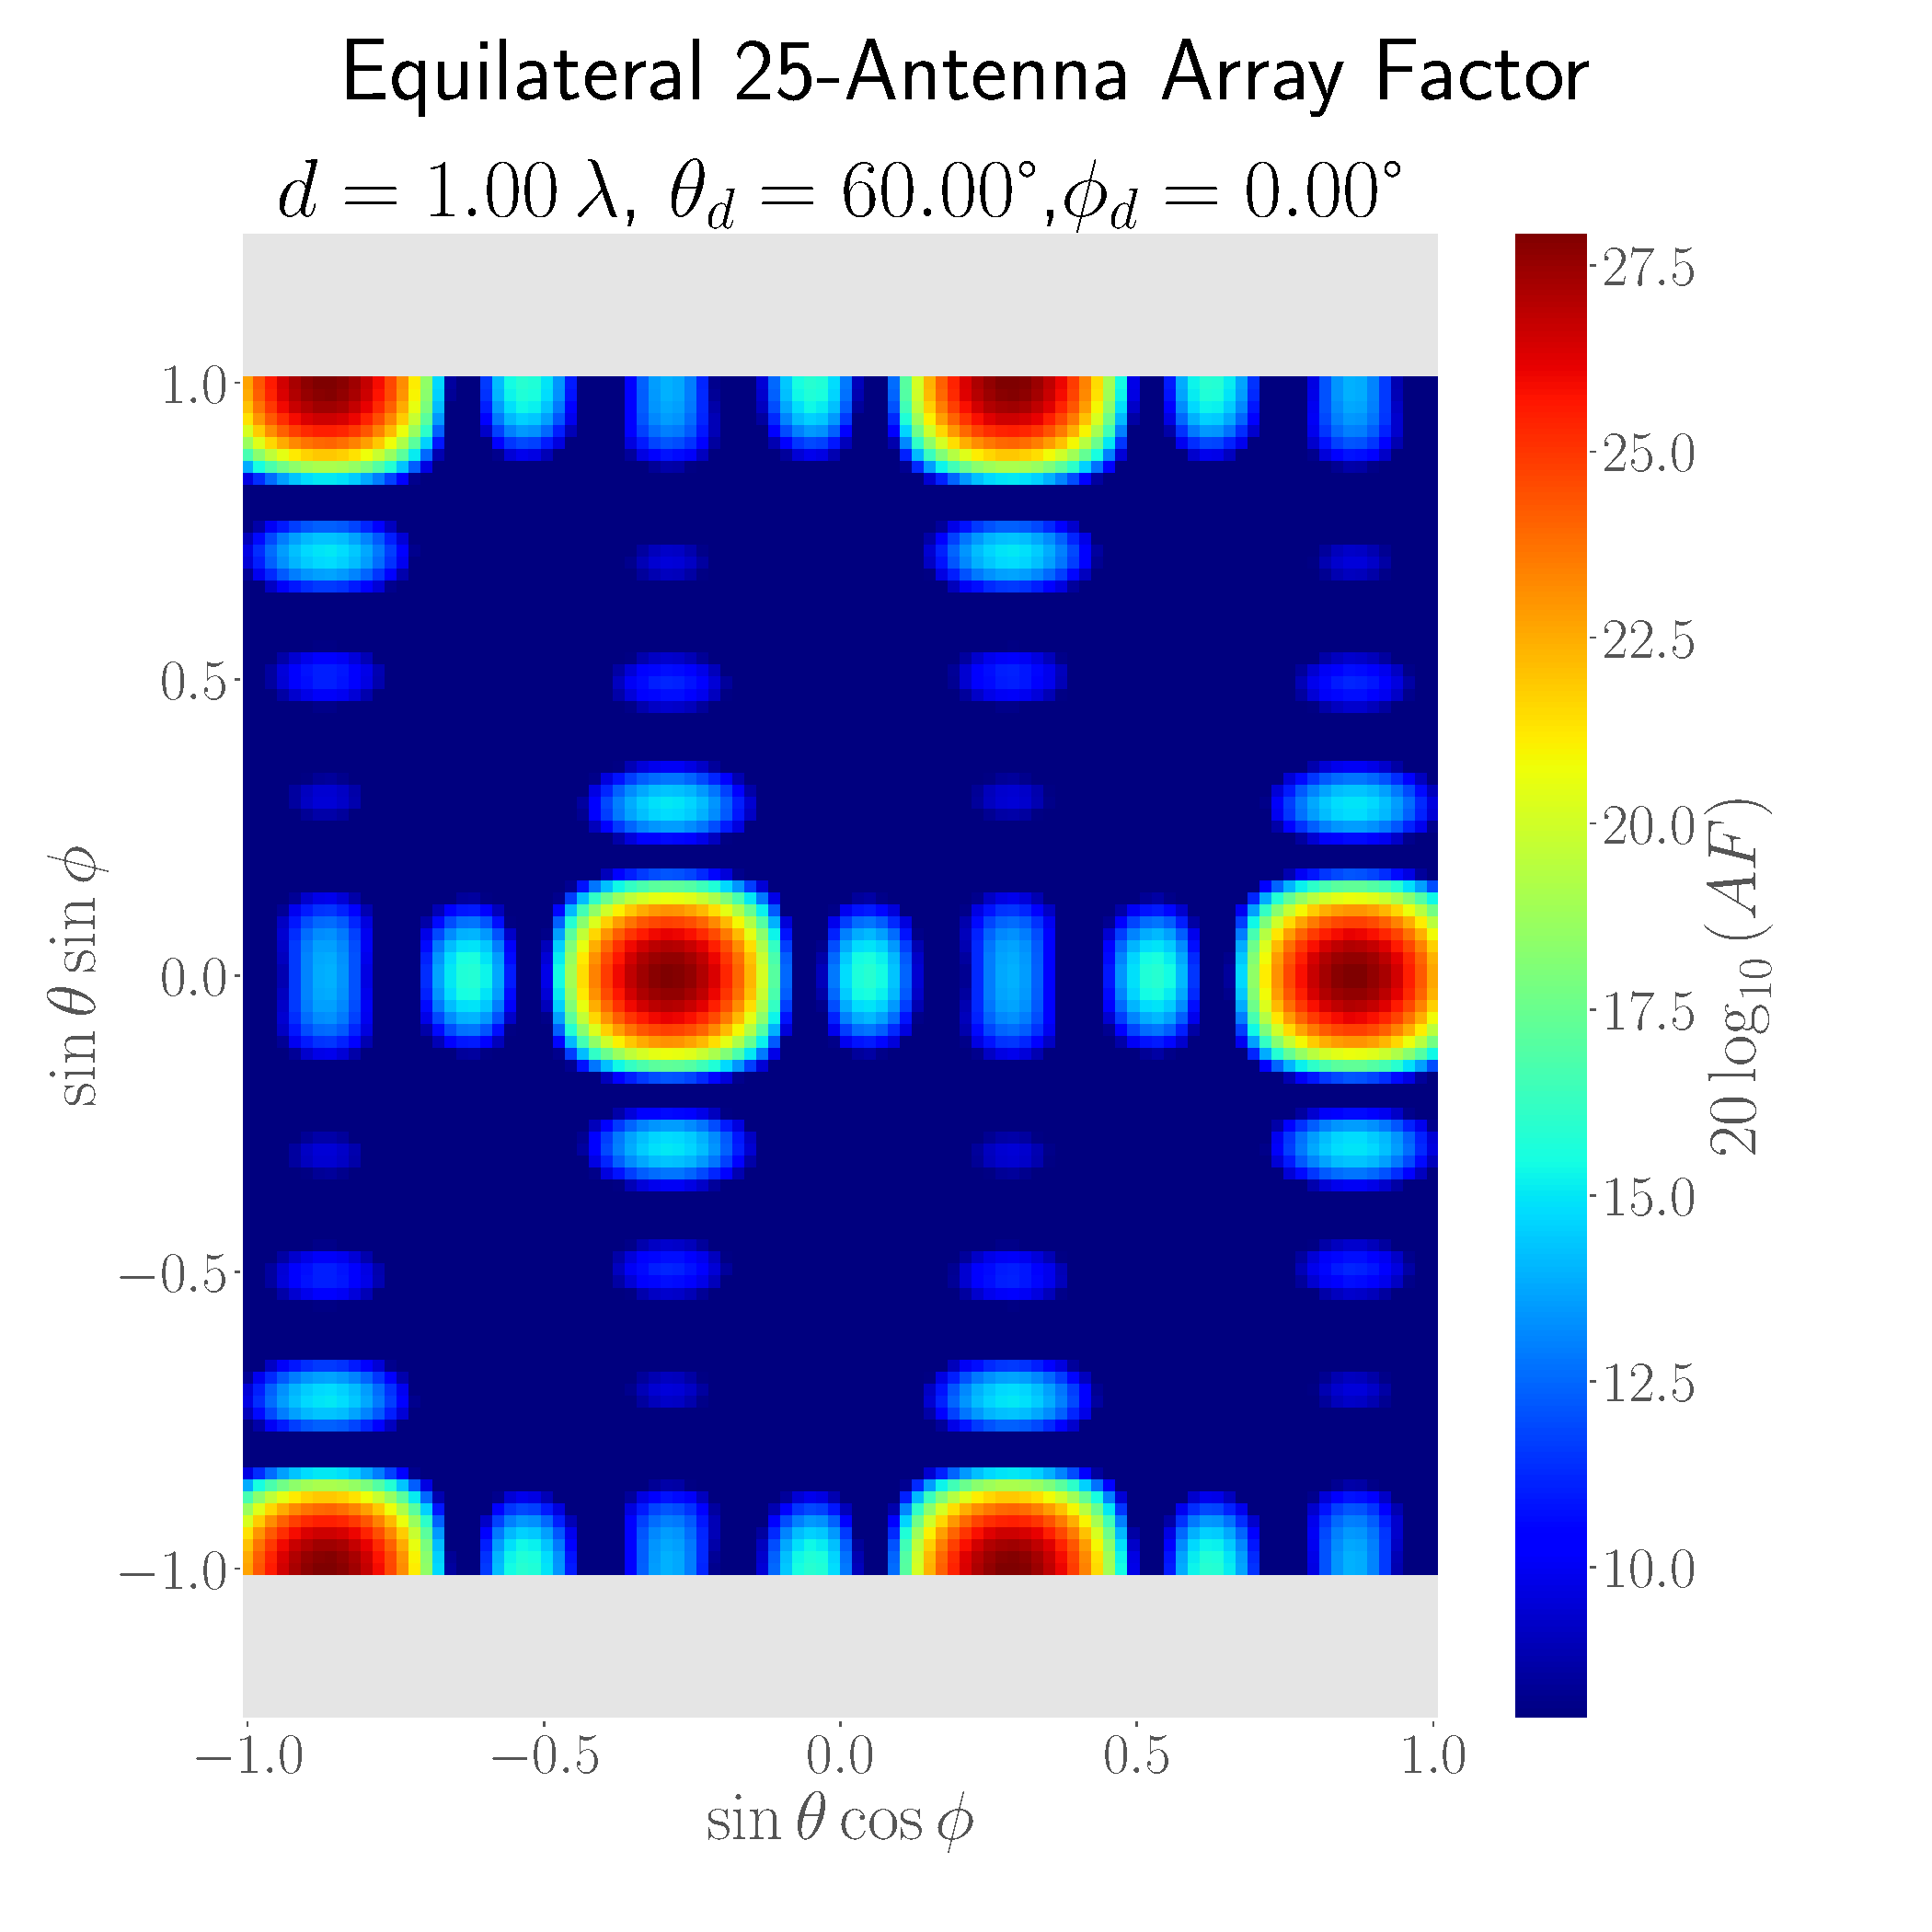
\includegraphics[width=\textwidth]{graphics/task_3/equilat-1.00-lambda-60.00-theta-0.00-phi-radpat.pdf}
    \caption{Equilateral off-vertically steered radiation pattern for $1.0\lambda$ spacing.}\label{fig:rad-equilat-1.0-60}
   \end{minipage}
\end{figure}

\begin{figure}[H]
  \begin{minipage}[t]{0.45\textwidth}
    \centering
    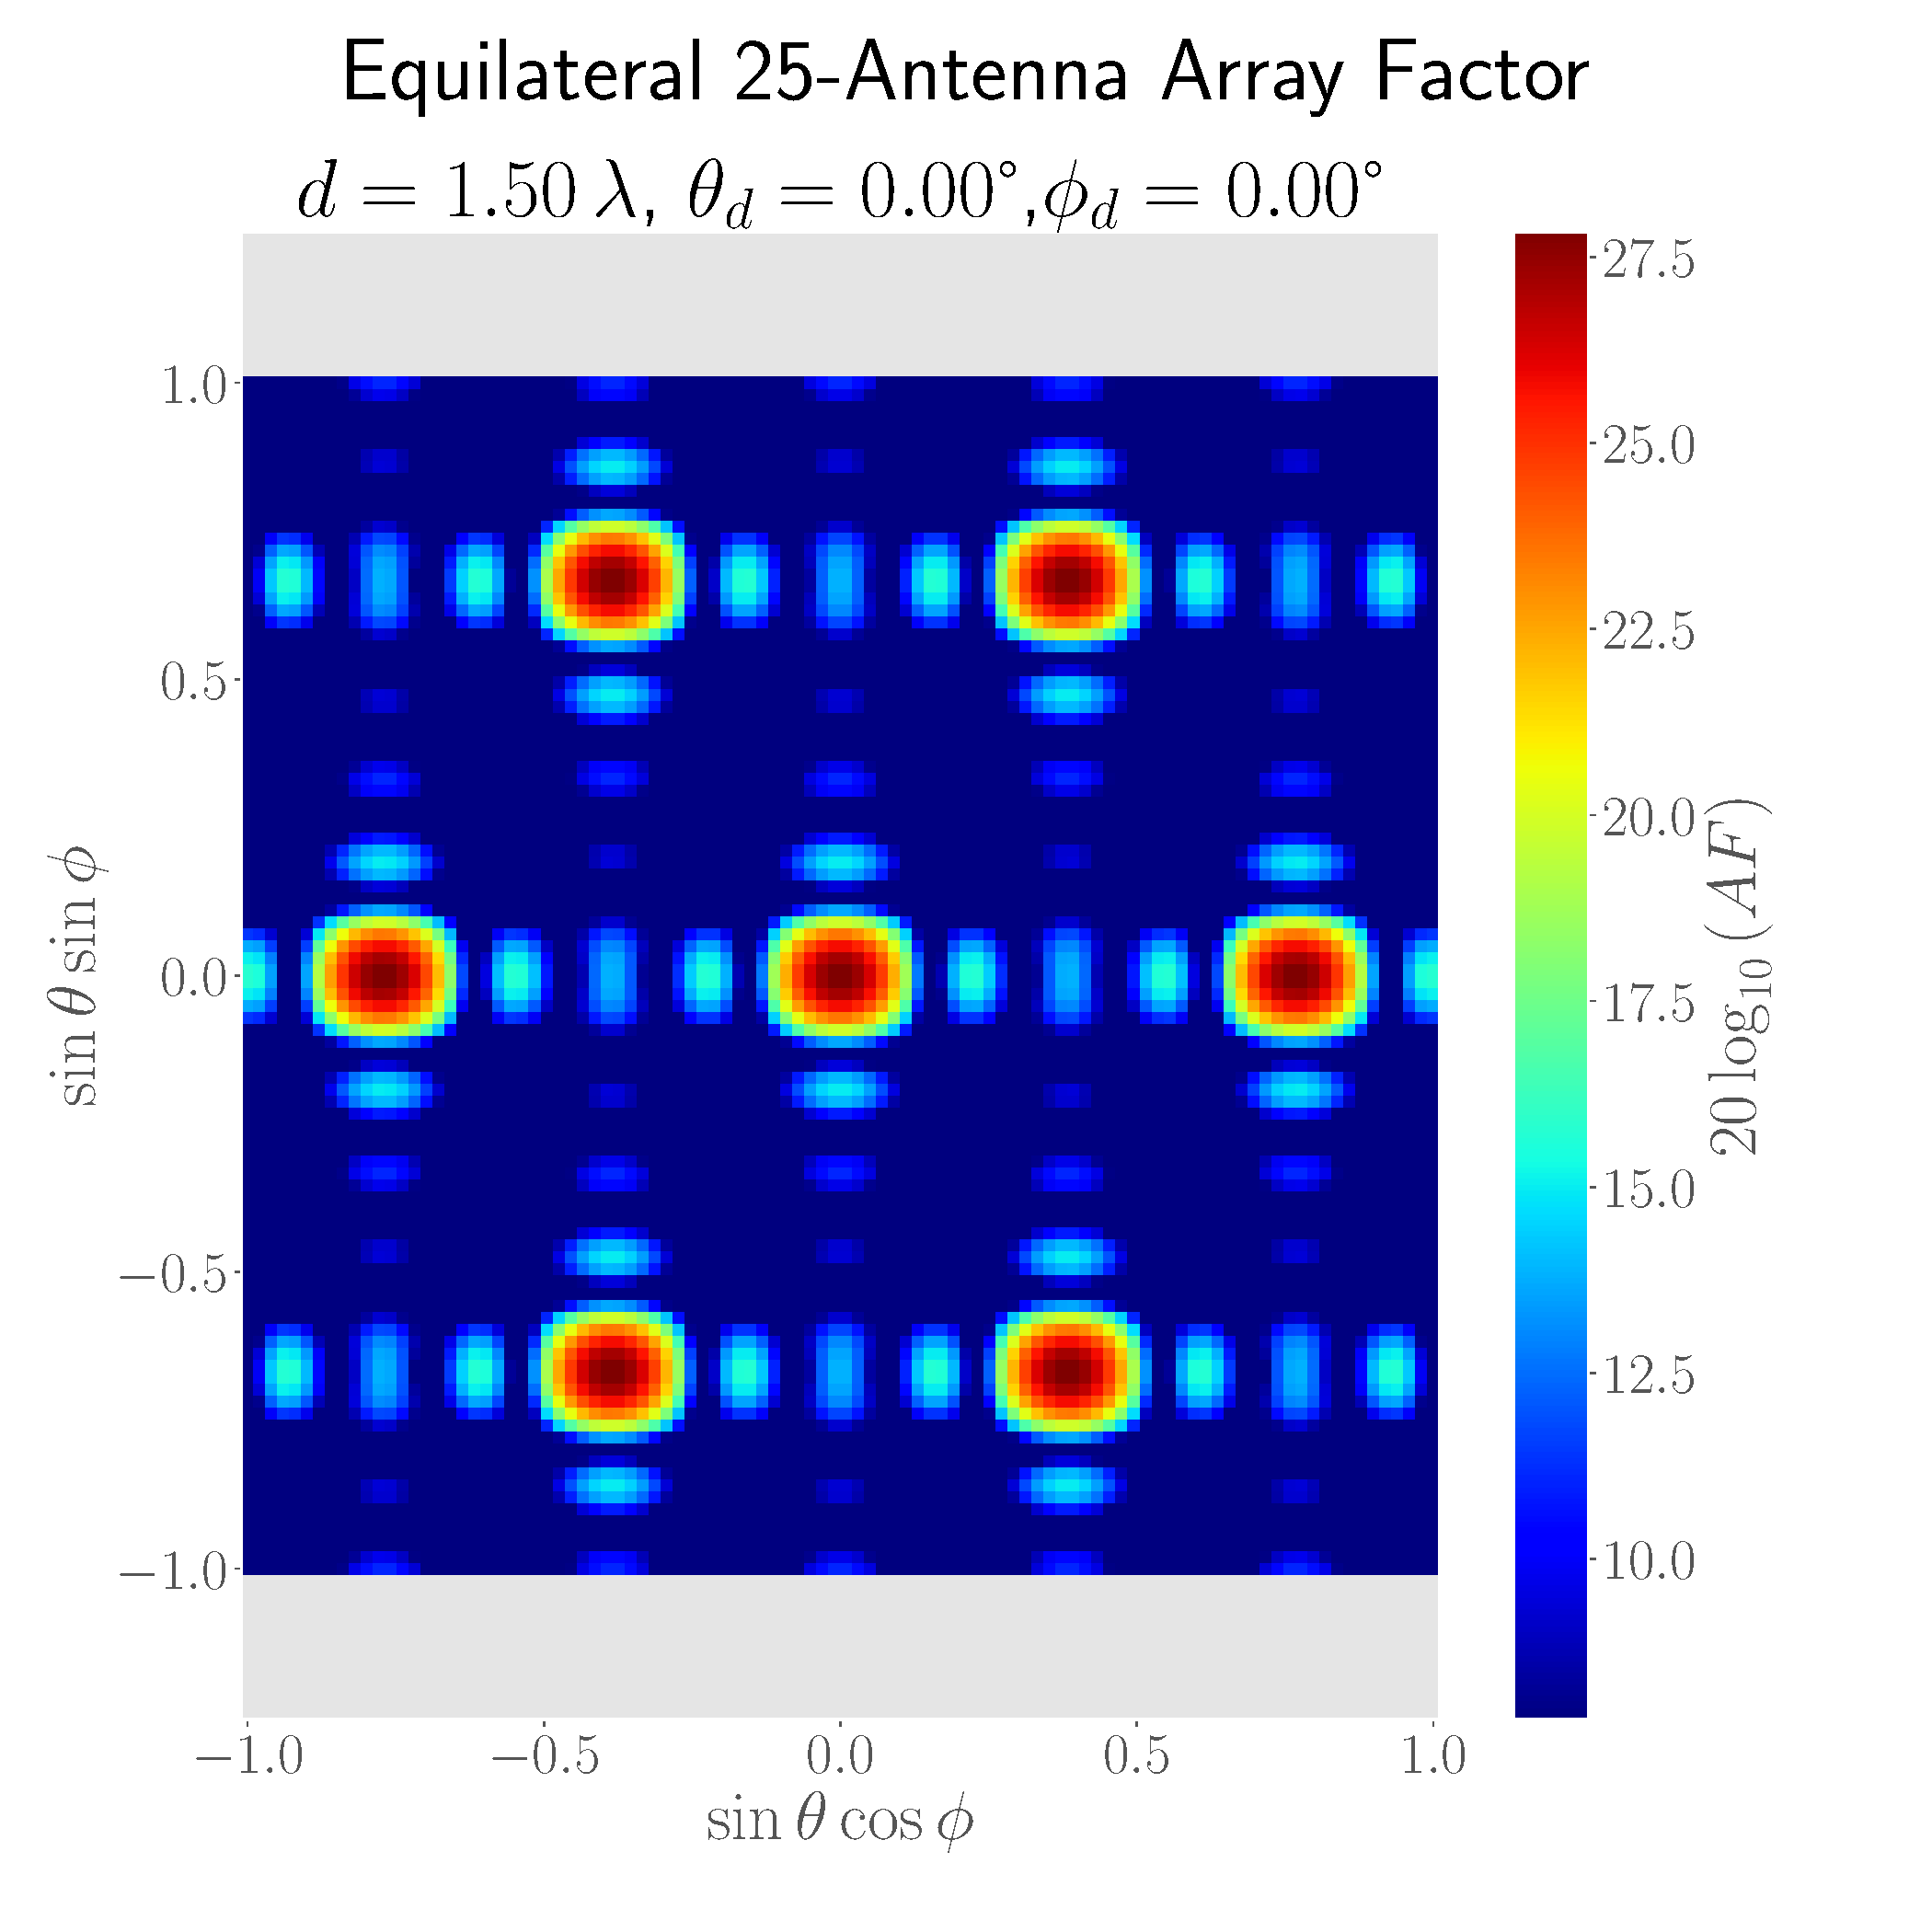
\includegraphics[width=\textwidth]{graphics/task_3/equilat-1.50-lambda-0.00-theta-0.00-phi-radpat.pdf}
    \caption{Equilateral vertically steered radiation pattern for $1.5\lambda$ spacing.}\label{fig:rad-equilat-1.5-0}
  \end{minipage}\hfill
  \begin{minipage}[t]{0.45\textwidth}
    \centering
    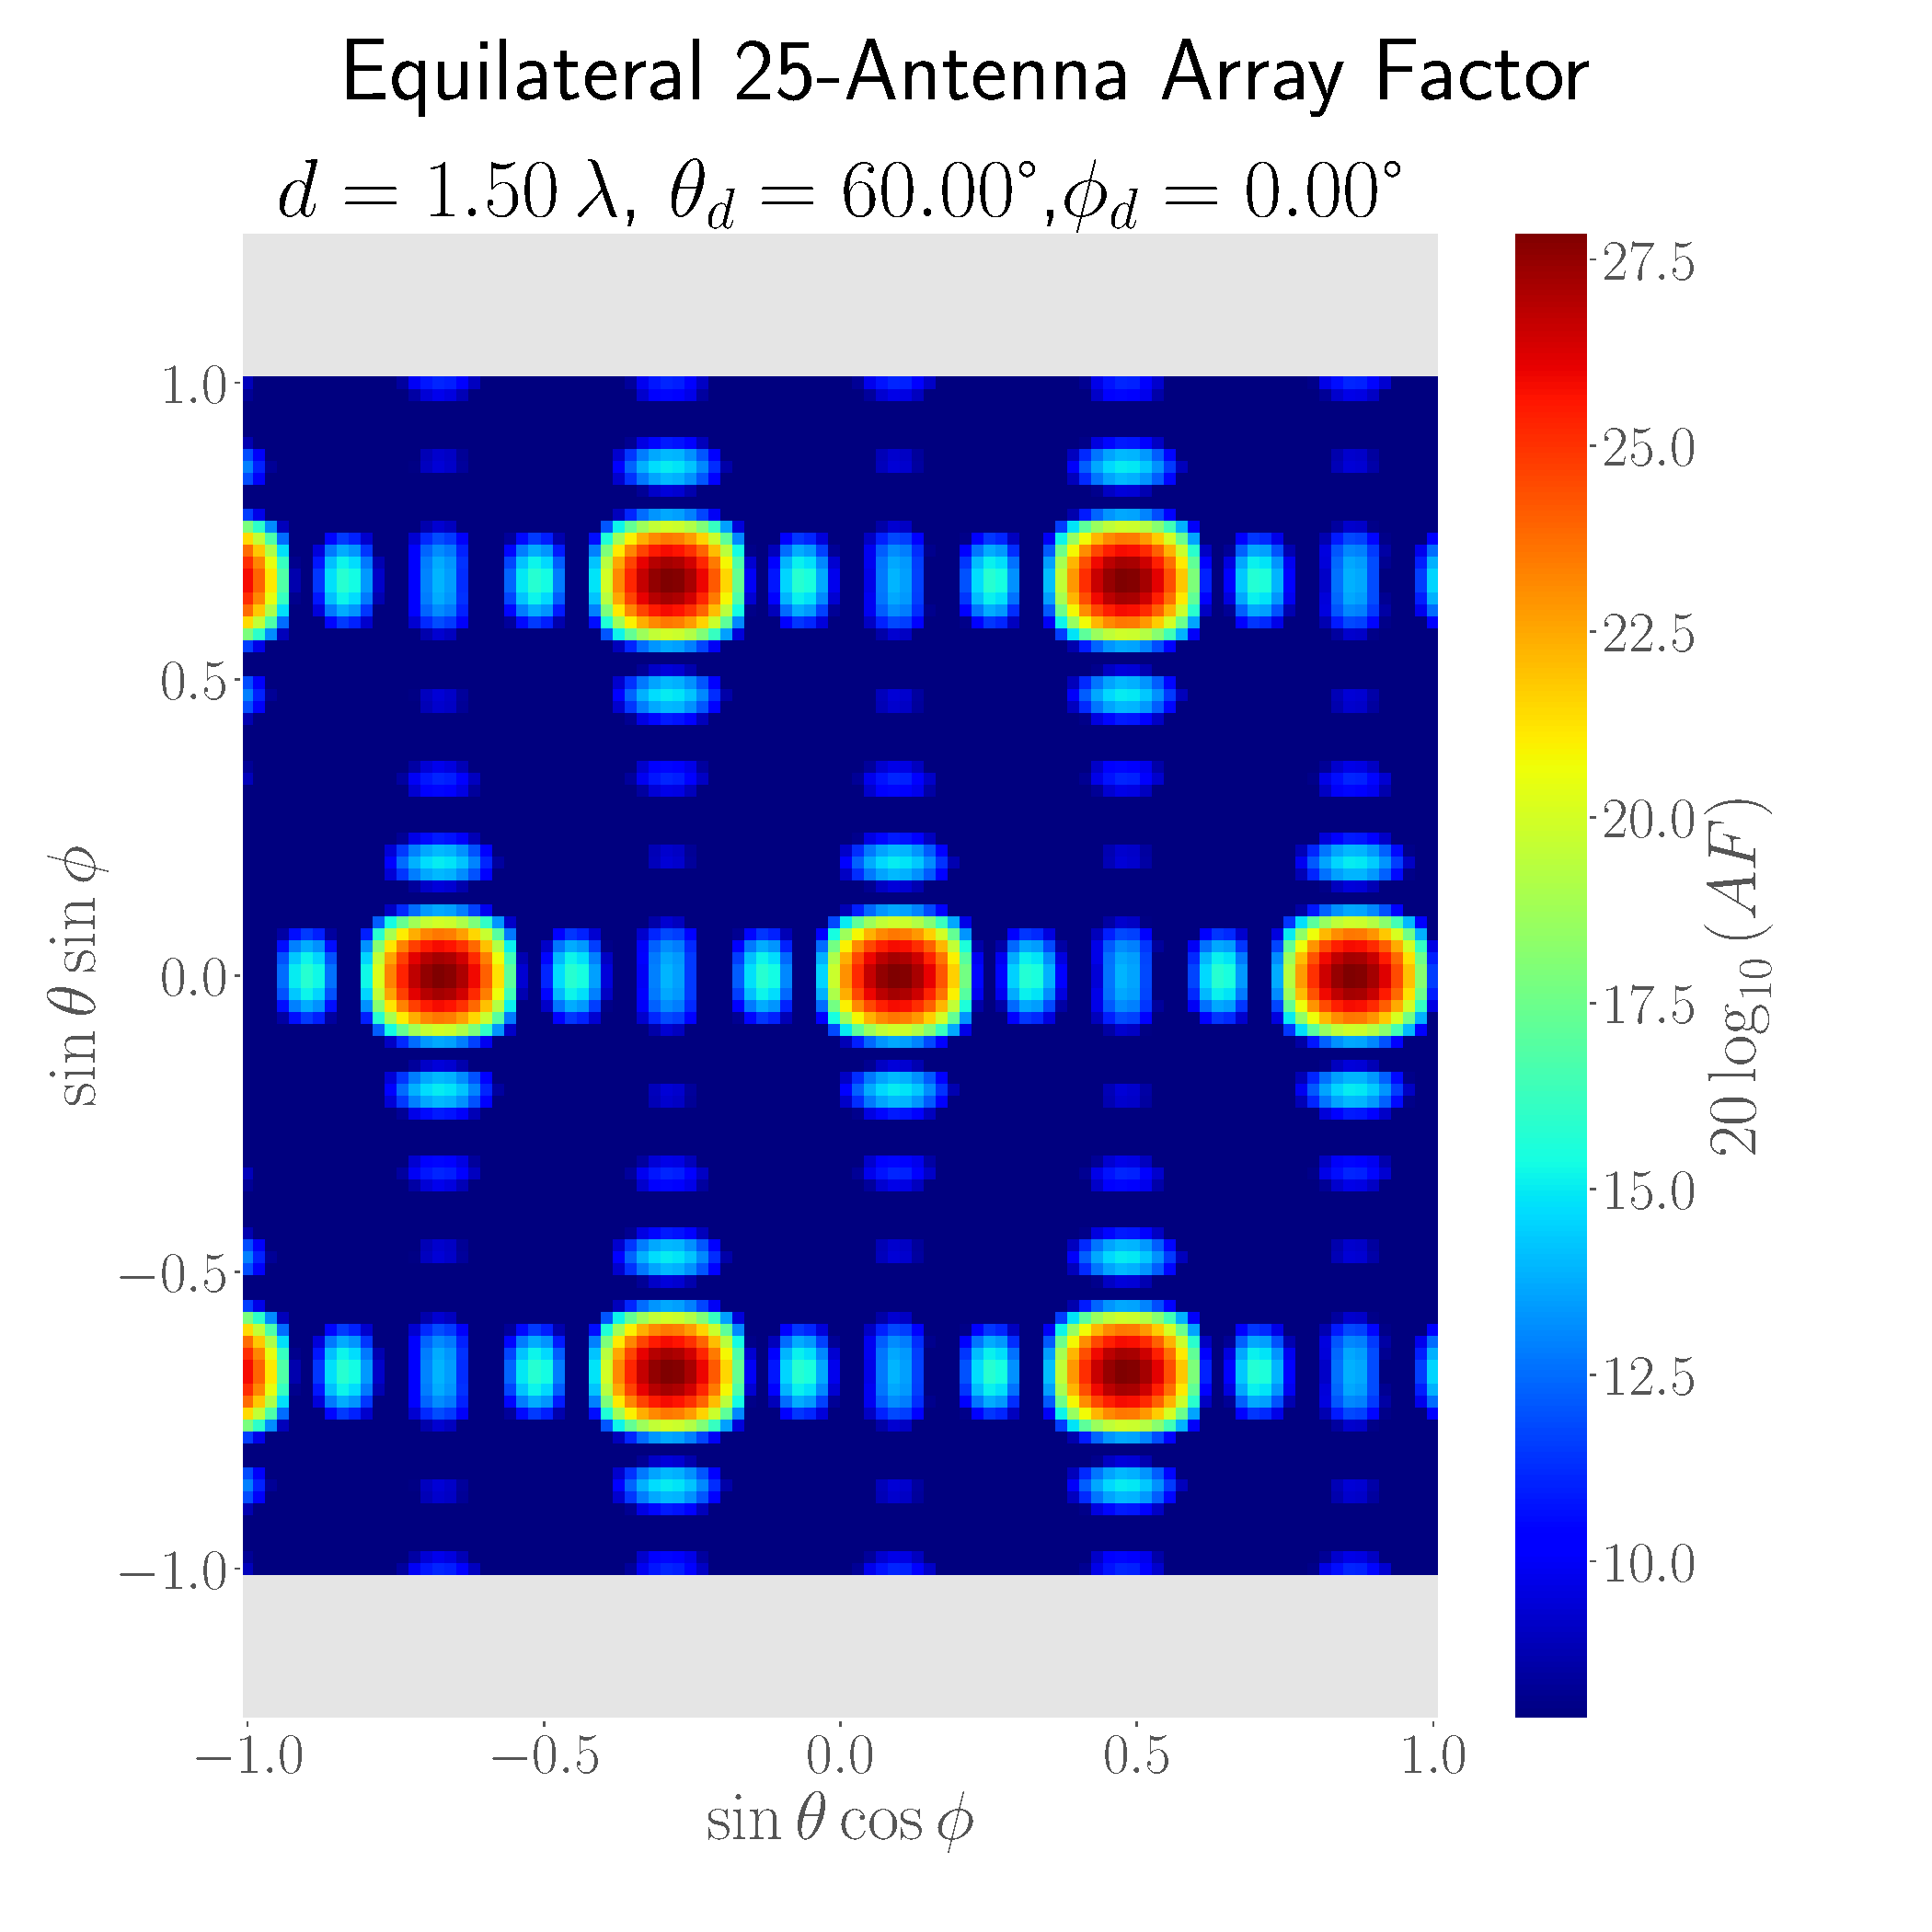
\includegraphics[width=\textwidth]{graphics/task_3/equilat-1.50-lambda-60.00-theta-0.00-phi-radpat.pdf}
    \caption{Equilateral off-vertically steered radiation pattern for $1.5\lambda$ spacing.}\label{fig:rad-equilat-1.5-60}
   \end{minipage}
\end{figure}


\begin{figure}[h]
    \centering
    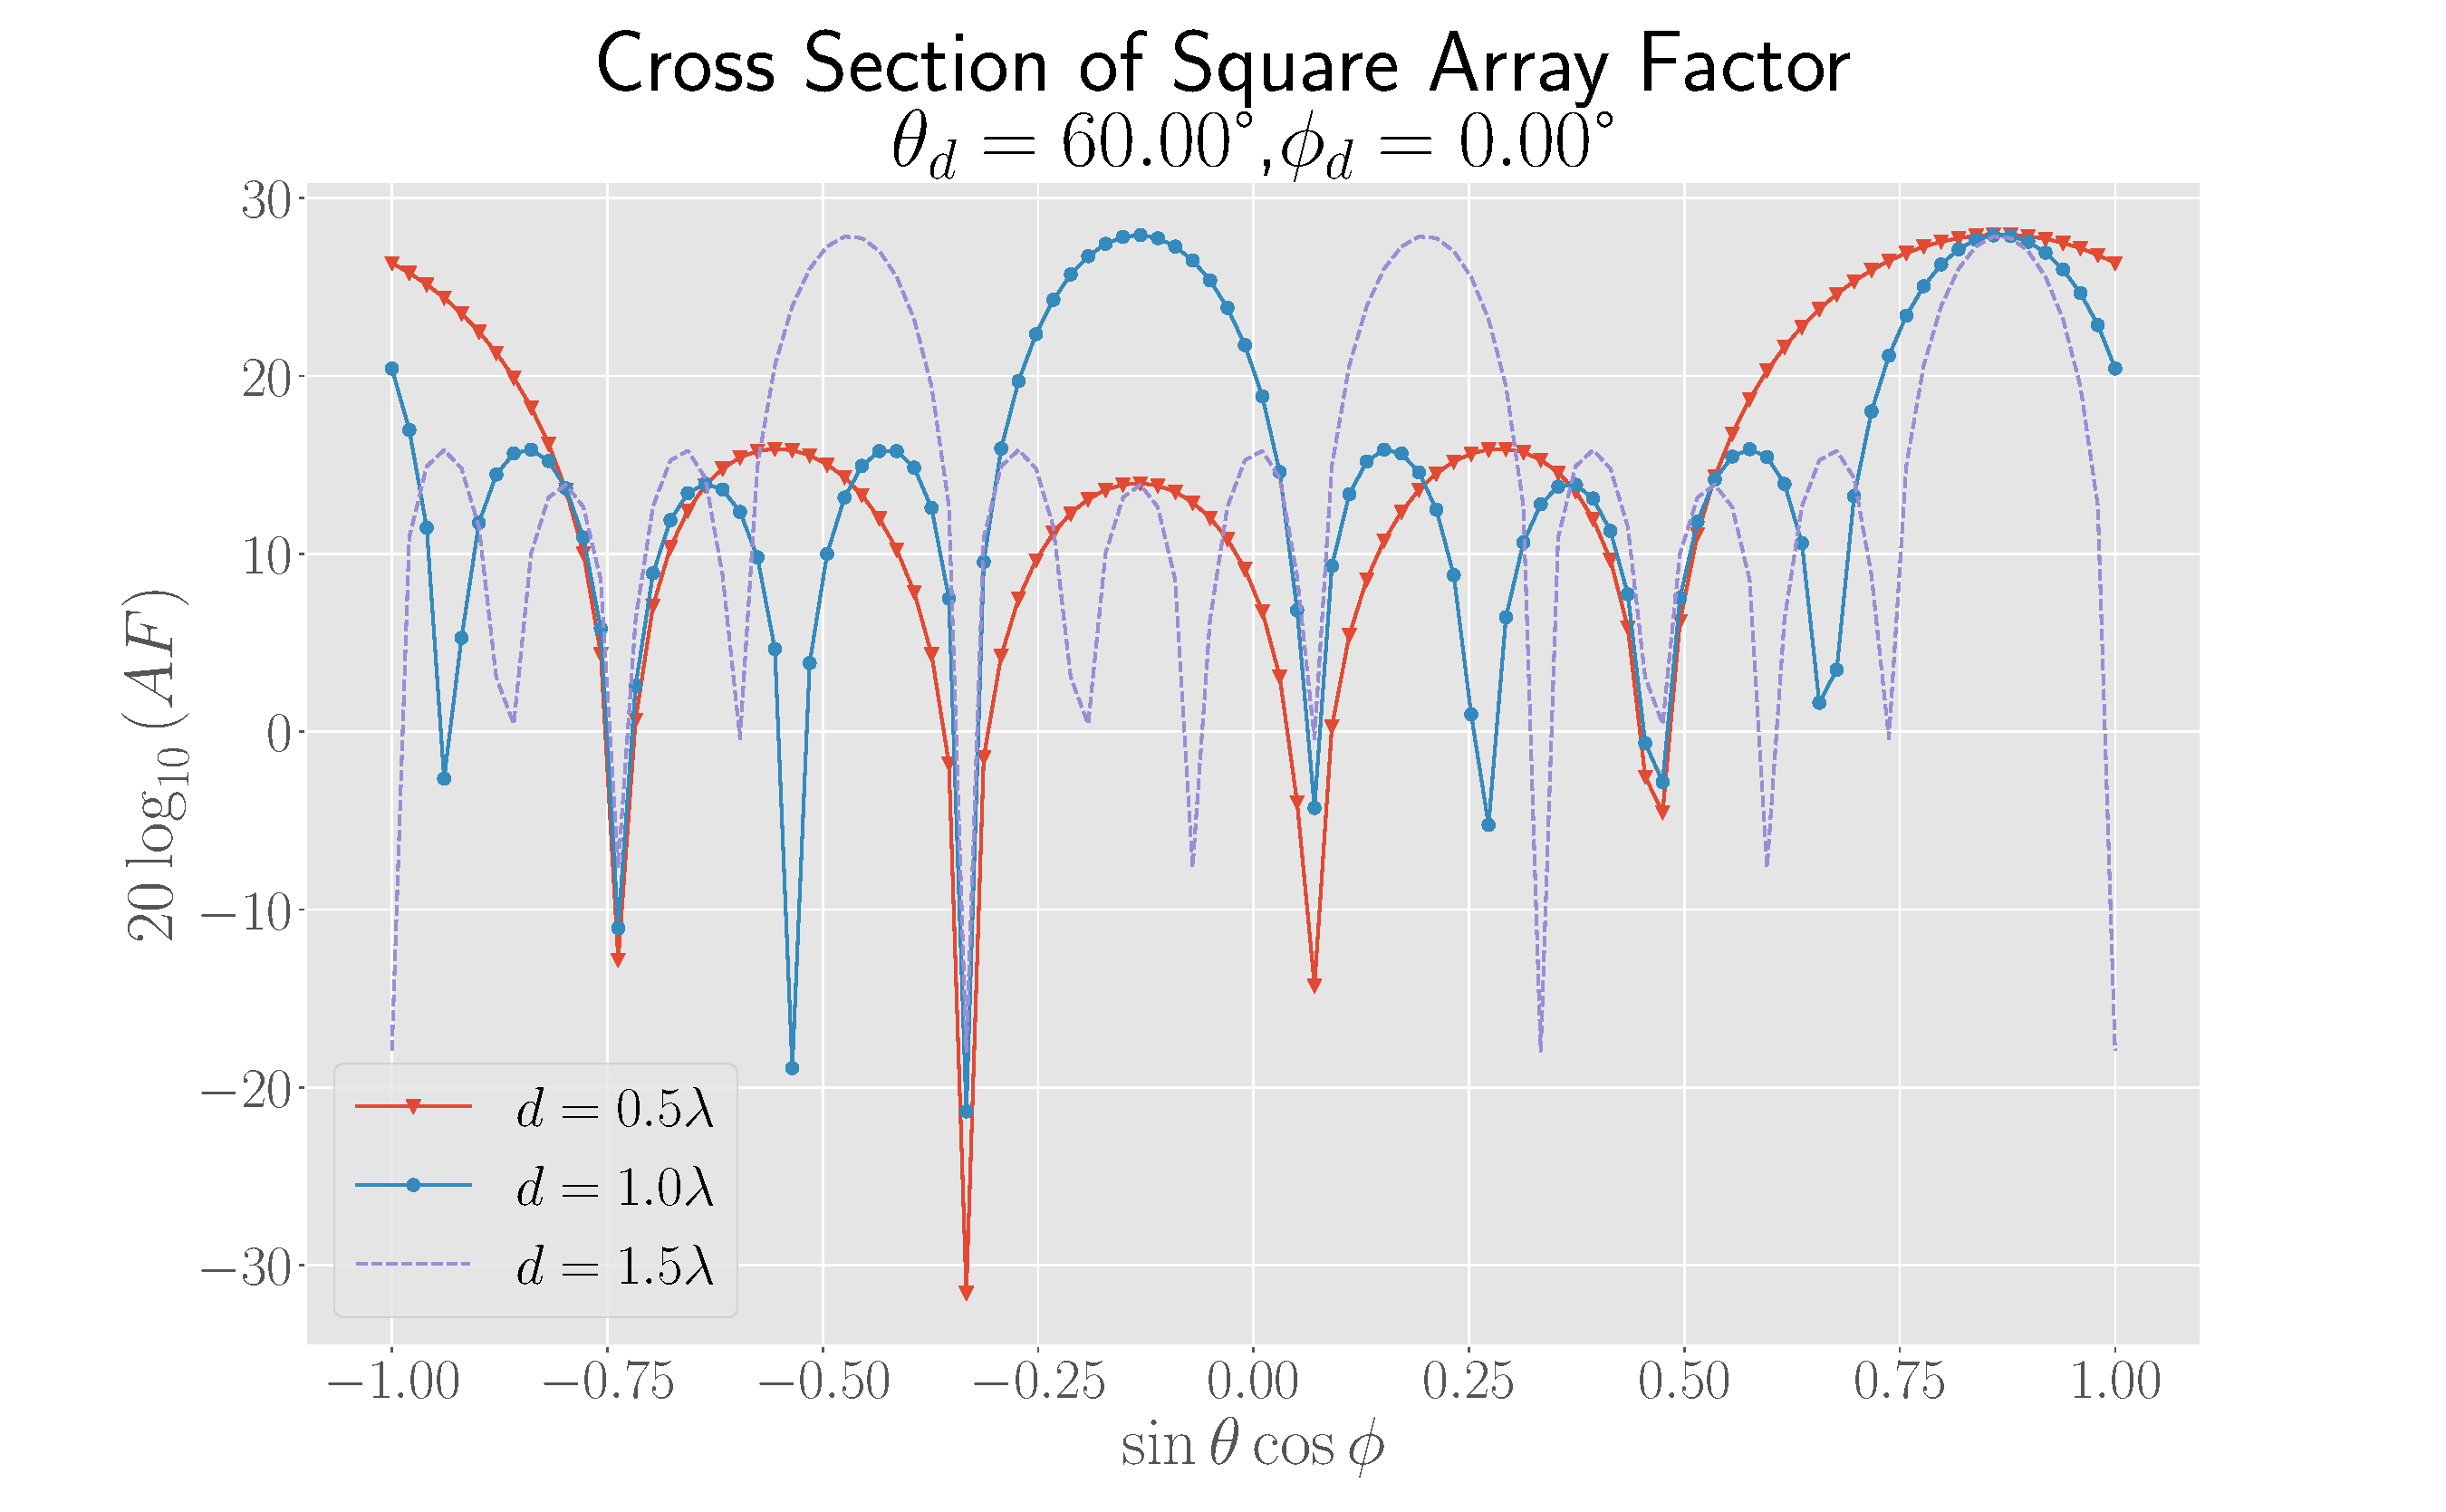
\includegraphics[width=0.618\textwidth]{graphics/task_1/square-60.00-theta-0.00-phi-cross.pdf}
    \caption{Comparison of cross-sections of the square array factor for different spacings.}\label{fig:square-cross}
\end{figure}


\begin{figure}[h]
    \centering
    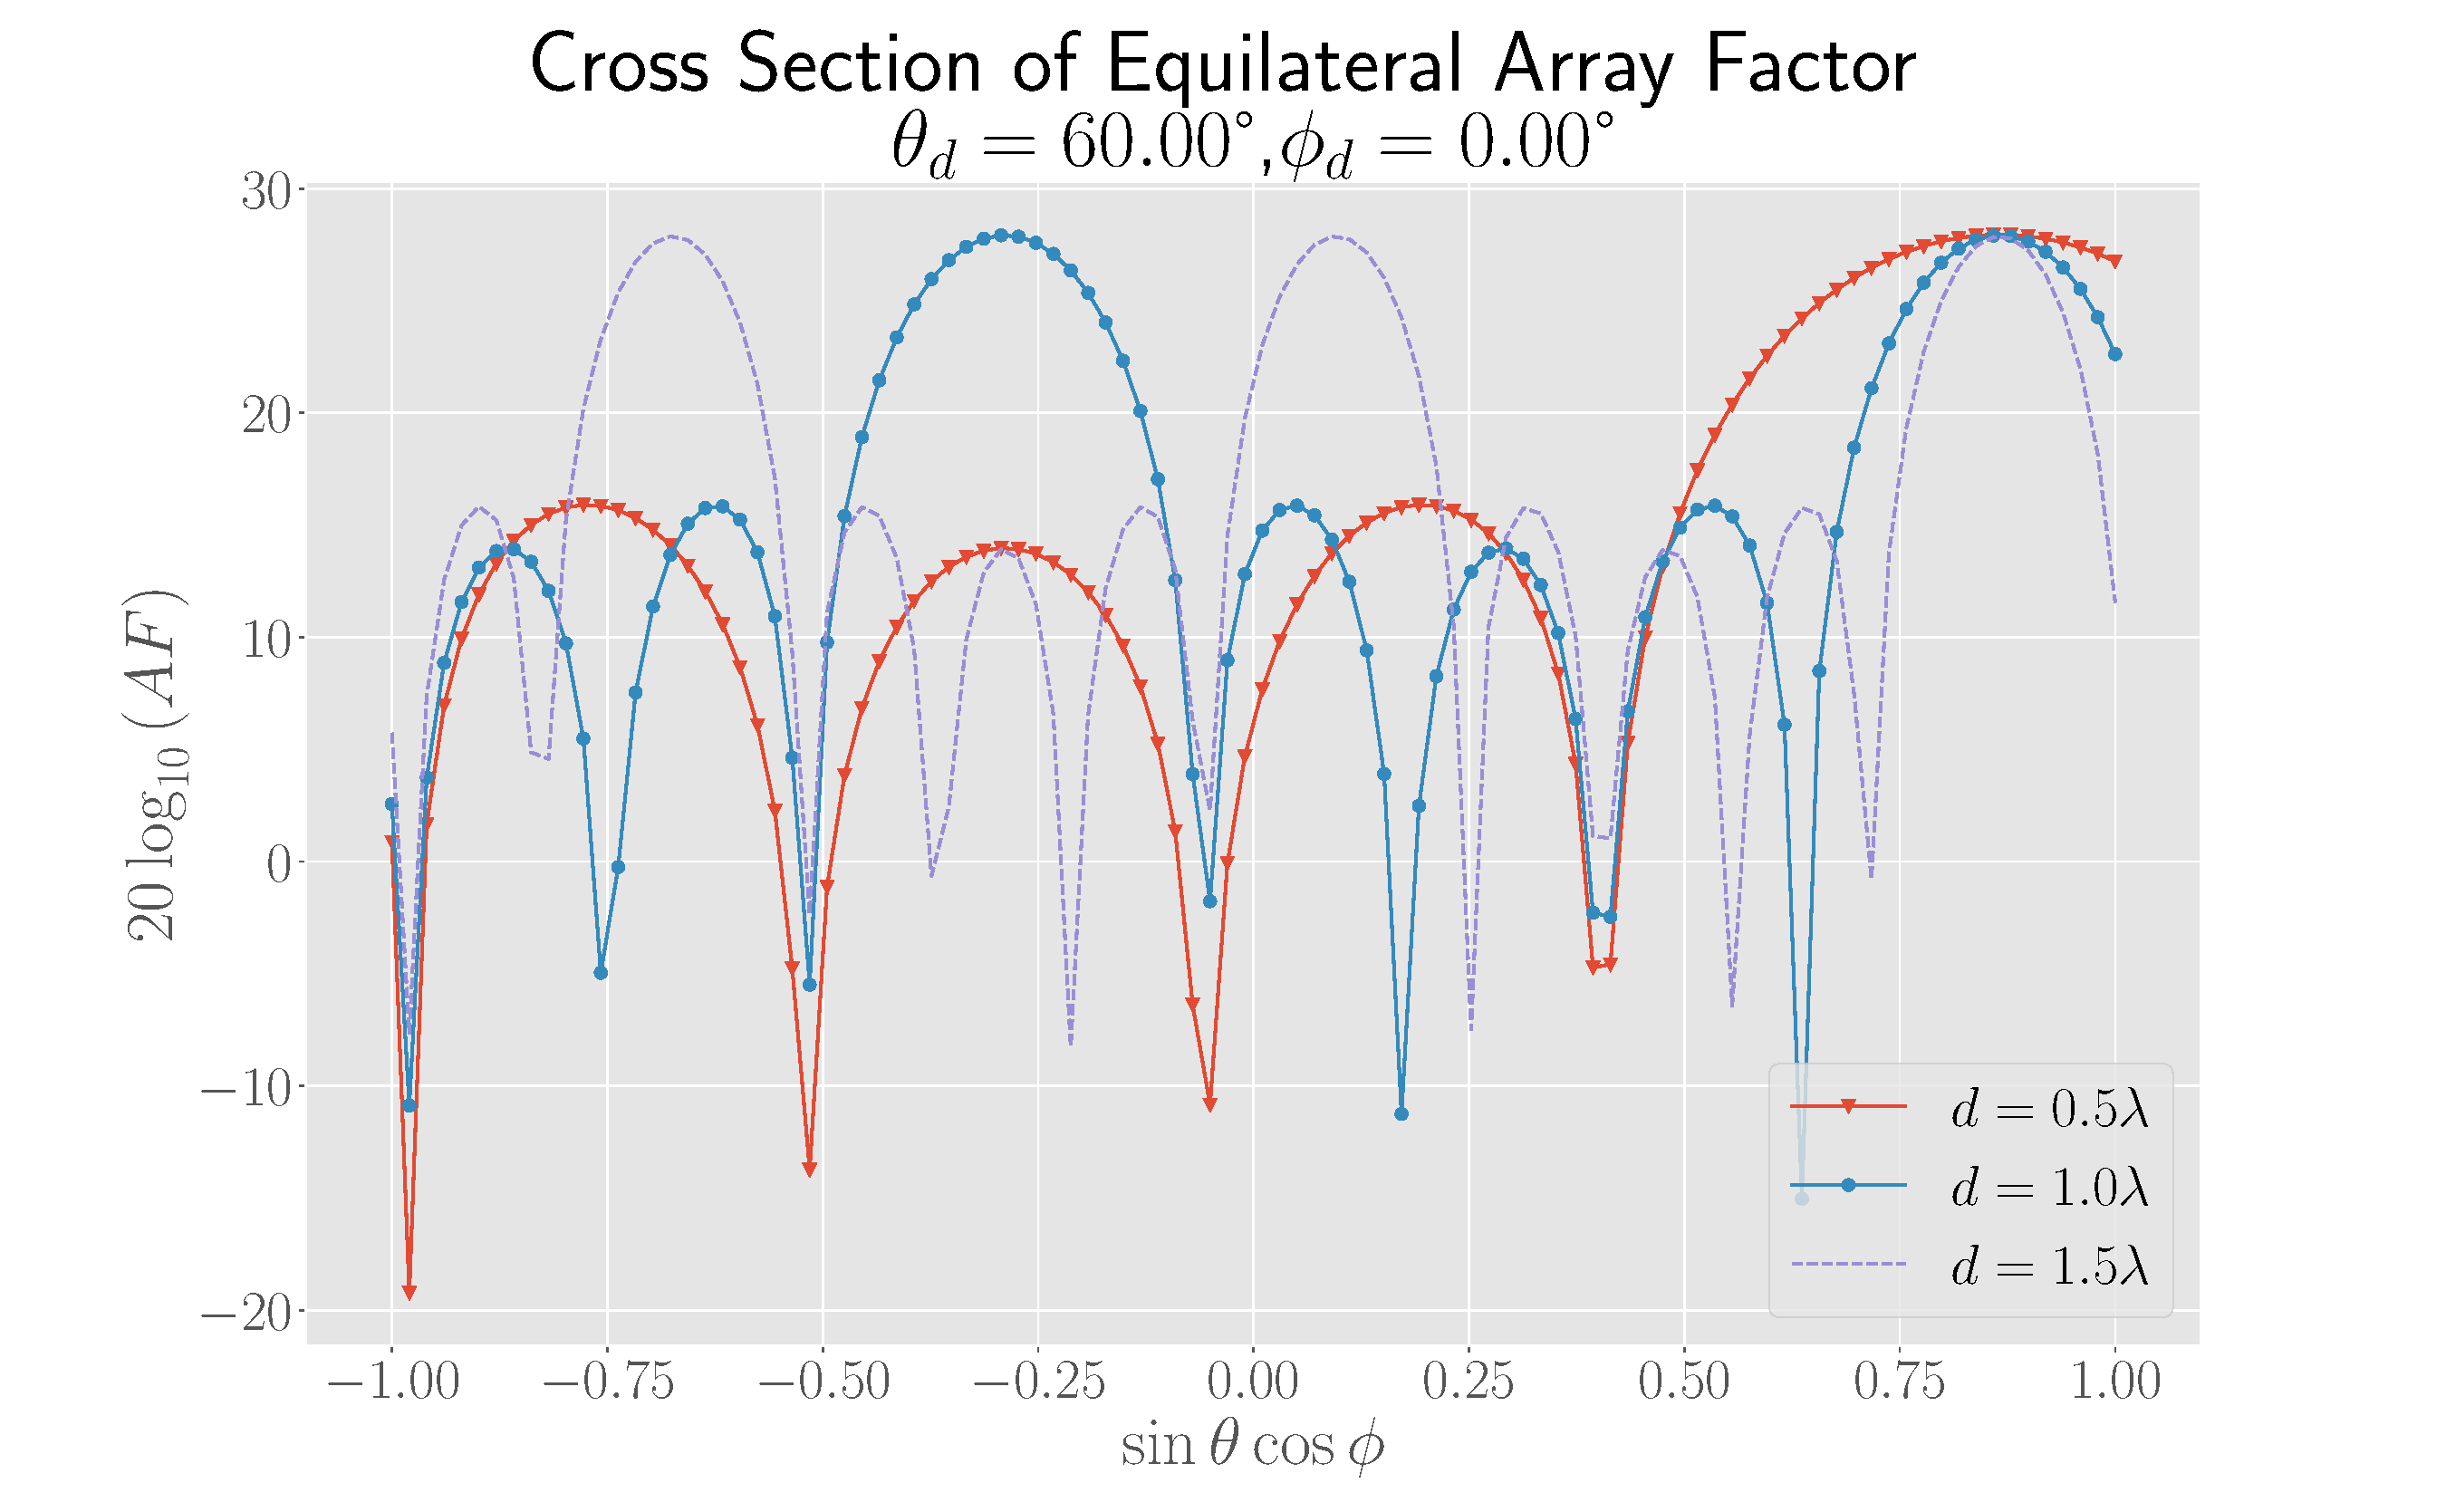
\includegraphics[width=0.618\textwidth]{graphics/task_3/equilat-60.00-theta-0.00-phi-cross.pdf}
    \caption{Comparison of cross-sections of the equilateral array factor for different spacings.}\label{fig:equilat-cross}
\end{figure}
